\chapter{Design}
\section{Data Flow Diagram}

\begin{figure}[H]
\centering
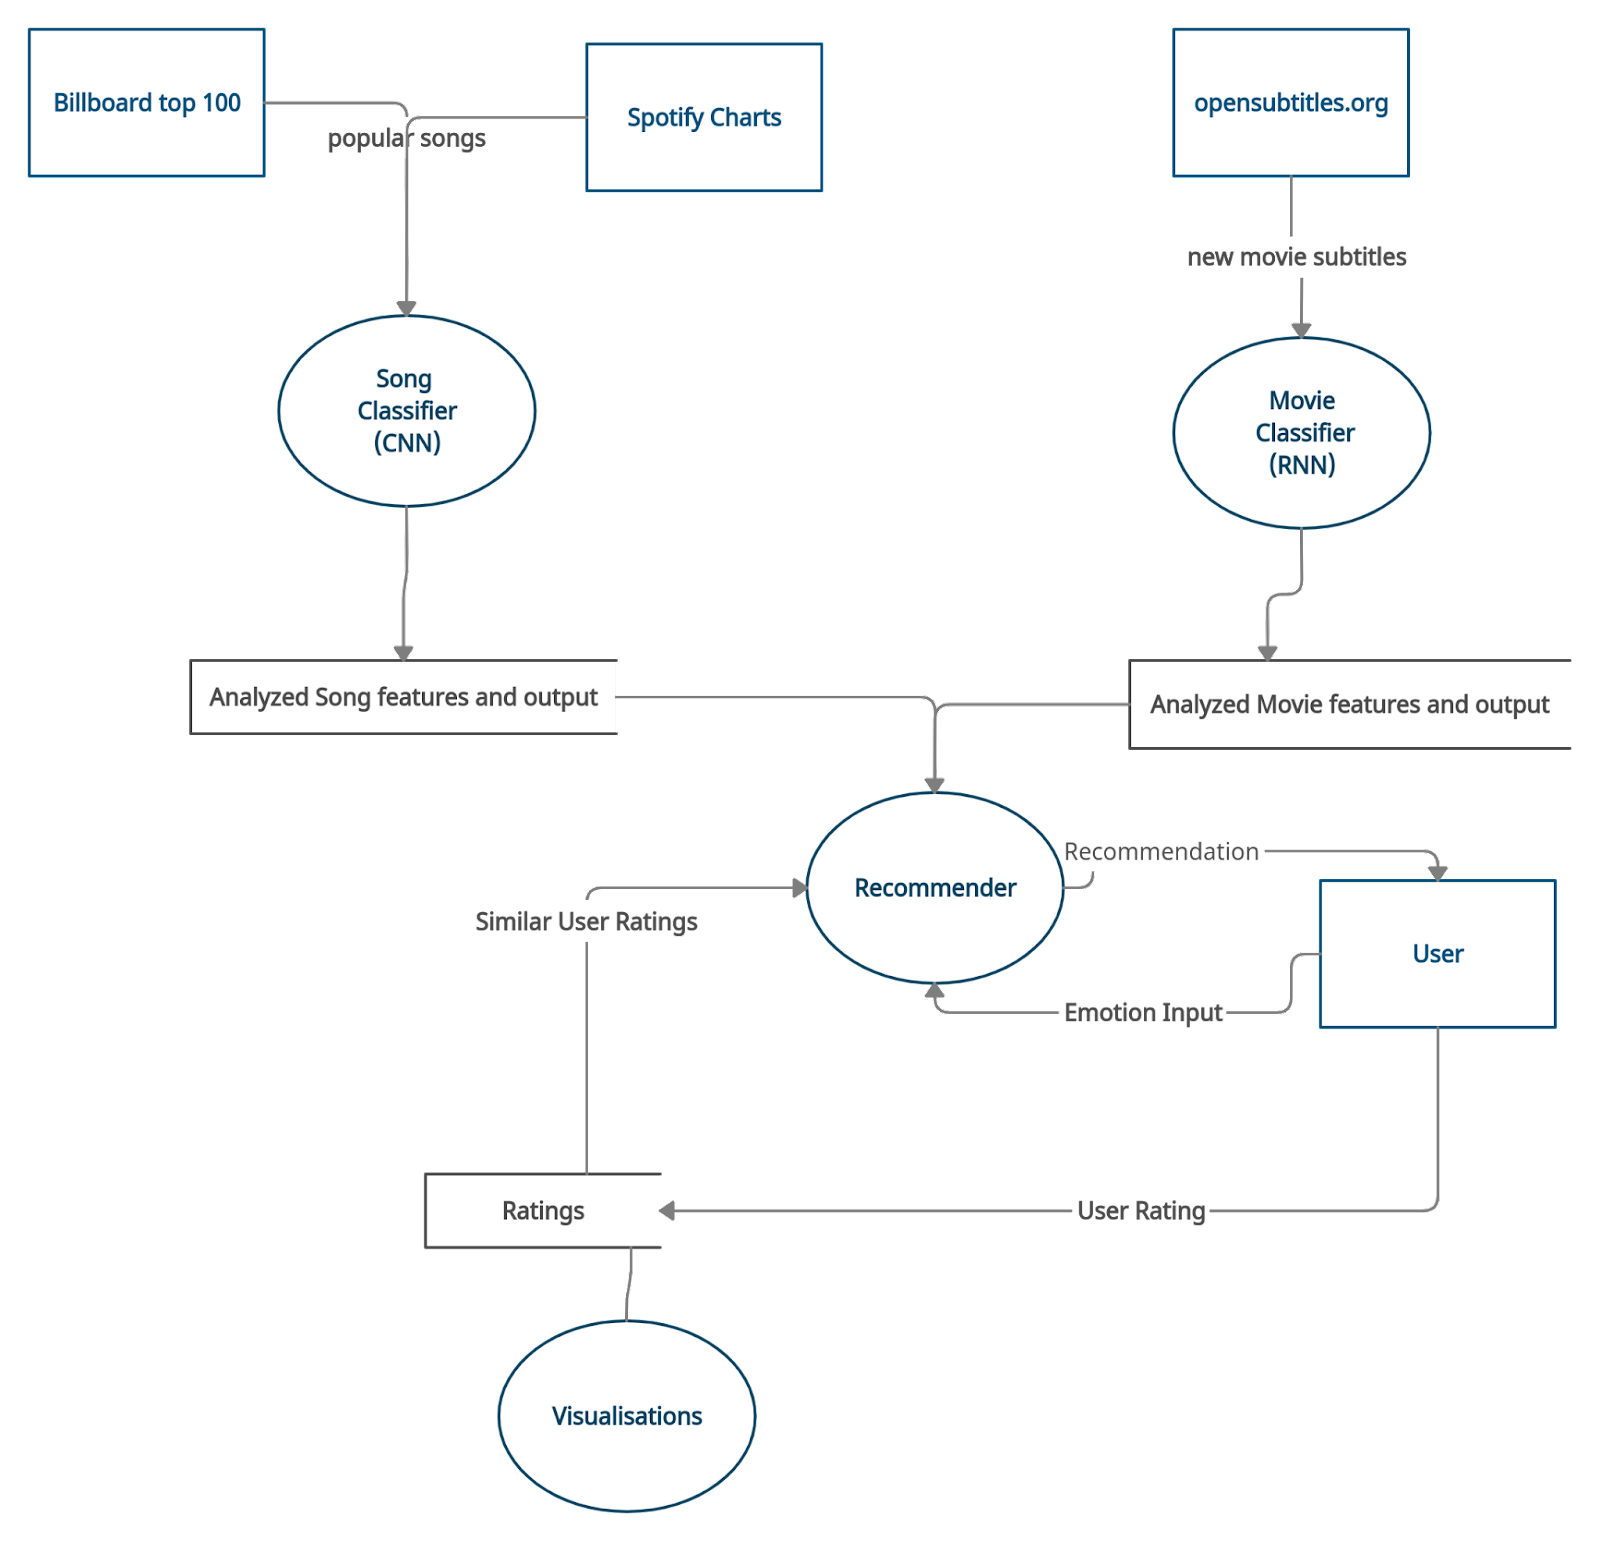
\includegraphics[scale=0.19]{imgs/dataFlowDiagram.png}
\caption{Data Flow Diagram}
\label{fig: data flow diagram}
\end{figure}

\section{ER Diagram}
\begin{figure}[H]
\centering
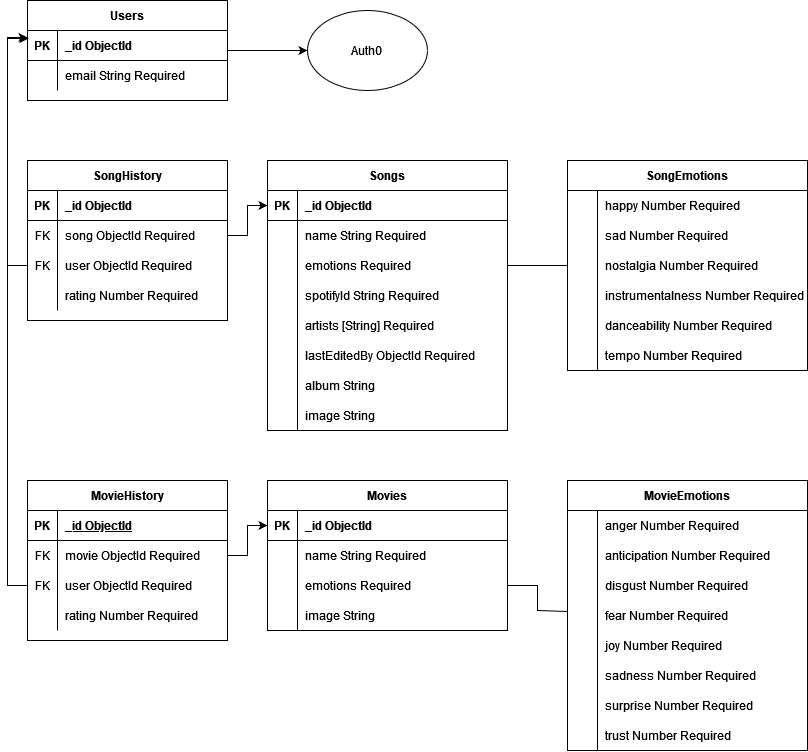
\includegraphics[width=\textwidth]{imgs/erDiagram.png}
\caption{ER Diagram}
\label{fig: erDiagram}
\end{figure}
For our app's class diagram (as shown in Figure \ref{fig: erDiagram} ), we have 5 entities. A unique ObjectId (\_id) attribute is common to all entities. In addition to this, each entity has the following attributes:
\begin{enumerate}

\item Users: The attribute email is of datatype String

\item SongHistory:
	\begin{itemize}
		\item The attributes song and user are of datatype ObjectId,
		\item The attribute rating is of datatype Number.
	\end{itemize}

\item MovieHistory:
	\begin{itemize}
	\item The attributes movie and user are of datatype ObjectId,
	\item The attribute rating is of datatype Number.
	\end{itemize}


\item Songs:
	\begin{itemize}
		\item The attributes name, spotifyId, album and image are of datatype String.
		\item The attribute emotions is an emdedded document containing attributes happy, sad, nostalgia, instrumentalness, danceability and tempo of datatype Number
		\item The attribute artists will be stored in an array of Strings.
	\end{itemize}

\item Movies:
	\begin{itemize}
		\item The attributes name, image are of datatype String.
		\item The attribute emotions is an emdedded document containing attributes anger, anticipation, disgust, fear, joy, sadness, surprise and trust of datatype Number
	\end{itemize}
\end{enumerate}

\section{Use case diagram}
A UML case diagram is the primary form of system/software requirements for a new software program underdeveloped. Use cases specify the expected behavior (what), and not the exact method of making it happen (how). Use cases once specified can be denoted both textual and visual representation (i.e., use case diagram). A key concept of use case modeling is that it helps us design a system from the end user's perspective. It is an effective technique for communicating system behavior in the user's terms by specifying all externally visible system behavior.

The main purpose of a use case diagram is to portray the dynamic aspect of a system. It accumulates the system's requirement , which includes both internal as well as external influences. It invokes persons, use cases and several things that invoke the actors and elements accountable for the implementation of use  case diagrams. It represents how an entity from the external environment can interact with a part of the system.
\begin{figure}[H]
\centering
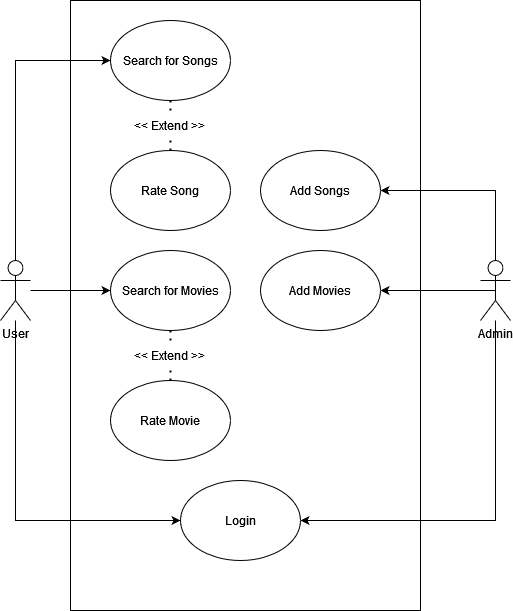
\includegraphics[width=\textwidth]{imgs/use_case.png}
\caption{Use case diagram}
\label{fig: usecase}
\end{figure}


For the use case diagram of our app (shown in Figure \ref{fig: usecase}), there are 2 actors (Someone who interacts with use case/triggers  the use case (system function)) - User and Admin. The ellipses/bubbles represent the system functions/use cases. \newline

The use cases we have for the users are:
\begin{itemize}
\item Search Songs
\item Search Movies
\item Login
\end{itemize}

The use cases we have for the admins are:
\begin{itemize}
\item Add Songs
\item Add Movies
\item Login
\end{itemize}

Extend relationship is used when a use case adds steps to another first-class use case. In our app, the user can choose to rate the song or movie if they are logged in and wish to do so. 
